\documentclass{article}
\usepackage[a4paper, total={7in, 9in}]{geometry}

\usepackage{graphicx} % Required for inserting images
% \usepackage[numbers]{natbib}


\usepackage{hyperref}
\usepackage{caption}
\usepackage{multicol}
\usepackage{amsmath}
\usepackage{tabularx}
\usepackage{easyreview}
\usepackage{comment}
\usepackage{tabularx}
\usepackage{tikz}
\usetikzlibrary{trees}
\usepackage{float}
\usepackage{multirow}
%\usepackage{svg}
\hypersetup{
	colorlinks=true,
	linkcolor=black,
	urlcolor=blue,
	citecolor=blue,
	pdfborder={0 0 0},
}

\usepackage{setspace} \singlespacing
\usepackage{enumitem}
\usepackage{fontspec}
\setmainfont{FreeSerif}
\setsansfont{FreeSans}
\setmonofont{FreeMono}
\usepackage{polyglossia}
\setdefaultlanguage{english} % Main language
\setotherlanguages{arabic, farsi, hindi, bengali}
\setmainfont{CMU Serif}
\newfontfamily\arabicfont[Script=Arabic]{Amiri}
\newfontfamily\hindifont[Script=Devanagari]{Lohit Devanagari}
\newfontfamily\bengalifont[Script=Bengali]{Lohit Bengali}
\newfontfamily\persianfont[Script=Arabic]{Amiri} % Persian can use the Arabic script font
\usepackage[backend=biber, style=numeric, maxnames=1, minnames=1]{biblatex}
\addbibresource{ref.bib}  % Assuming your .bib file is named references.bib

\title{Automated Essay Scoring in Arabic and Low-Resource Indic Languages: A Systematic Literature Review}
%\author{Ahmad Shafiq Zia, Swardiantara Silalahi}
\date{September 2024}

\begin{document}    
	
	\maketitle
	\section{Introduction}
	Automated Essay Scoring (AES), also known as Automated Essay Grading (AEG), Automated Essay Evaluation, utilizes specialized computer programs to assign grades to written texts in educational settings. Fundamentally, the goal of AES is similar to the traditional method of scoring, which involves training a human rater to interpret and apply a rubric to evaluate students' responses.\\
	
	AES models can be designed to evaluate either short-form responses - also known as Automated Short Answer Grading (ASAG) - or essay-style answers, with the latter being more complex. This increased complexity arises from the open-ended nature of essays, making it challenging to evaluate them using a single model answer. Additionally, considerations of various features, such as essay structure, coherence, and style, further complicate the evaluation process. \\
	
	The development of effective AES models necessitates extensive work with Machine Learning (ML) and Natural Language Processing (NLP) to account for the unique characteristics of free-text answers. Majority of models utilize syntactic and/or semantic features. Most models are built on supervised learning, where labeled datasets are needed to train them.
	\\
	AES systems significantly enhance the efficiency of grading free-text student responses, particularly in standardized testing and online learning environments. These systems can serve various purposes: they can act as independent assessors of student scores, function alongside human examiners, or monitor the ratings provided by examiners. In cases involving a large number of online learners submitting free-response answers, such as those on popular  MOOC and course platforms with millions of learners, AES system can not only save time but also reduces costs by minimizing the need for human examiners. \\
	
	These systems can provide faster speeds and lower costs for grading large volumes of student essays. Furthermore, they can help reduce biases and unreliability that examiners might have \cite{malouff2016bias} and study has also been done in addressing rating biases in training datasets for such models. \cite{amorim2018aesbias}.\\
	
	On the downside, though, AES systems may require substantial time and financial investment. To achieve high accuracy and reliability, large datasets need to be prepared. Models might also be inaccurate in cases where writing styles may be unique. In some cases, reliability issues may arise since certain aspects of essay, such as assessment of creativity of ideas and propositions is challenging to implement. Overall, the lack of transparency might be questioned by test-takers. If the rules used by the model are publicly released, critics concern that test-takers might exploit these rules to achieve significantly higher scores from the AES system than they would receive from human examiner. \\ 
	\subsection{Working of an AES system}
	In our collection of papers, we observed that majority of papers tend to follow a similar approach in implementing their model.
	\begin{enumerate}
		\item \textbf{Preprocessing} \\ The raw text is transformed and modified into a format that can be used by the AES system. This can include removing noise, normalization. Extra features not needed for the next stage are removed as will. This can include removing features like stop words, lemmatization, stemming, tokenization and other techniques utilized in NLP text preprocessing
		
		\item \textbf{Feature Extraction} \\ Various features are extracted from preprocessed data. There are two typical approaches that can be utilized for feature identification and extraction. \\ The first being manual extraction of features from the text. The model looks to extract a predetermined set of features through the text, and then calculates to deliver a final score using those features as variables. However, such models can be more inaccurate than those which automatically extract features. Deep learning based models learn to automatically identify features in order to increase accuracy of the predictive score. They consist of several hidden layers in the neural network, hence making it harder to identify the complex features they use.
		
		\item \textbf{AES Model} \\ Model is trained using machine learning on the features extracted in Step 2. Some employ  Machine Learning, or Deep learning algorithms to learn the relation between the extracted text features and the essay score in the training dataset. This step utilizes the statistical yields and weights. Some models use a hybrid approach, combining traditional and machine learning methods.
		\item \textbf{Scoring} \\ A test dataset can include essays that are either based on specific prompts or are of a generic type. This dataset is used to generate scores for the essays. Additionally, the work involves normalizing or scaling these scores to align with the scoring standards of human examiners.
	\end{enumerate}
	After the score is generated, the model is evaluated by comparing the generated scores on the test dataset against the human examiner scores, and correlation / accuracy is measured.
	\subsection{Development of AES Systems in English Language}
	The earliest development of Automated Essay Scoring (AES) started in 1996 with the Project Essay Grader (PEG) by Ellis Paige \cite{page2003peg}, which provided scores based on features like grammar, word choice, and word length and vocabulary etc. The model works by extracting such textual features, and trained to determine the grade using the best predicted combination of the weighted features. The features used in the model were considered to be indirect predictors of writing quality. Therefore, the model was vulnerable to cheating. \\ Further work was done to implement AES systems that could extract features directly contributing to the writing quality. One such work was the Intelligent Essay Assessor in 1999 \cite{foltz1999essayassessor}, which used Latent Semantic Analysis (LSA). This statistical approach identified the association among the words in a topic. This ability to determine semantic similarity helped determine the quality of the essay by comparing it against a similar text of known quality. Thus, it could detect plagiarism and was more fool-proof than PEG. \\ The E-rater Intellimetric (2006) \cite{rudner2006intellimetric} and the Bayesian Essay Test Scoring System (BETSY) \cite{rudner2002bayes} also utilized NLP-based techniques. Much work has been done in employing various other techniques, including deep learning, and leveraging transformer-based models like DeBERTa \cite{susanto2023deberta}. These trends can provide an insight into the development of AES models and different methods being adopted over time. \textcite{ramesh2022review} have conducted a thorough review of AES in the English language. \\
	Furthermore, education systems in many US states have integrated AES systems in their testing. This includes Utah Compose Tool, and Ohio standardized test. 
	
	
	
	\subsection{Development of AES in Foreign languages}
	Development of AES systems in other languages depends on various factors because of the popularity of that language and the unique opportunities and challenges that language might present. Each language has different set of grammatical, and morphological rules. Therefore, they have variations in syntactic and semantic aspects of language.
	Majority of languages other than English have less resources and fewer studies. This can be due to many factors, including less number of speakers compared to popular languages (like English) or are less commonly taught in education.
	To address these challenges, work is also being done to develop multilingual models, for example,  by translating text into English for scoring. The study \textcite{firoozi2024bert} is such an example. 
	\begin{figure}
		\centering
		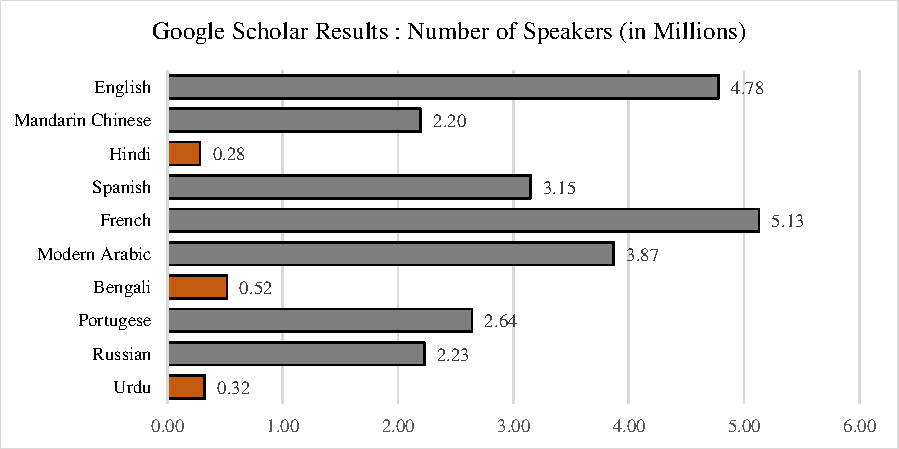
\includegraphics[width=\textwidth]{img/ratio.pdf}
		\caption{Google Scholar Results with the search query: \\
			\textit{"Automated Essay Evaluation"OR"Automated Essay Scoring" (name of language)}}
		
		\label{searchresult}
	\end{figure}
	Different language families have distinct linguistic features, which can impact how AES systems are implemented in languages belonging to those families. The classification of language families is inherently variable and not universally agreed upon. Therefore, the discussion presented here should be regarded as a generalization, focusing primarily on well-known and widely spoken languages. \\
	Figure \ref{searchresult} Shows the ratio of the number of results for a Google Scholar Search query number to the number of language speakers \cite{wikitotalspeakers} in top 10 most spoken languages. It is assumed that given a larger number of speakers of a certain language, there will be more language learners (native and non-native). While Google Scholar does not always present relevant search results, the statistic can be, however, used to provide an estimate of the development of AES systems in the respective languages. The search results show that despite a large number of speakers, Many languages, especially Indic, have a surprising lack of work done. This can be attributed to various reasons like the lack of existing NLP related resources, or lack of existing datasets. \\
	While individual languages in a family can differ in various ways, a lot of features can be common. For example, all languages in Sino-Tibetan family (Chinese, Mandarin, Burmese etc.) share a logo-graphic writing system. \\
	On the other hand, the Indo-European language family is the largest and most diverse, comprising of numerous branches with distinct characteristics. Each branch within the Indo-European has a variety of unique features while sharing some common root vocabulary and fundamental language construction.\\
	
	This paper reviews the development of widely spoken Indo-Iranian (Indic) languages from the Indo-European Family and Arabic from the Semitic Family. These languages have been chosen because of their unique linguistic challenges and personal familiarity with these language groups.
	These include:
	\begin{enumerate}
		\item Arabic
		\item Persian
		\item Hindi
		\item Bengali
	\end{enumerate}
	While existing literature review on Automated Essay Scoring (AES) is focused on Arabic \cite{litreviewarabic}, this paper aims to expand the review by including recent studies on both Arabic and Indic languages, find trends of different methods and trends as well as their potential to be used in other low-resource languages.
	%\newpage
	\section{Research Method}
	\subsection{Research Questions}
	Our review will evaluate each paper on the basis of following research questions:
	\begin{enumerate}[label=\textbf{RQ\arabic*}, leftmargin=1.5cm]
		\item What are the datasets available for AES systems in the selected languages?
		\item How did the paper deal with preprocessing?
		\item What features were used by the paper and the model utilized?
		\item What were the drawbacks and advantages of the utilized models?
	\end{enumerate}
	\subsection{Search Process}
	Well-known computer science repositories including ACM, IEEE Xplore, Springer, Science Direct, ACL were searched with publications from 2010 to date 2024. \\
	The search strings included ``Automated Essay Scoring", ``Automated Essay Evaluation", ``Automated Essay Grading", ``AES", ``Automated Answer Scoring"  with name of the language in the search query. Due to limited number of papers found, additional searches were made through Google Scholar, and preprints like Archiv as well.
	\\
	\subsection{Selection Criteria and Quality Assessment}
	The searched papers then went through an inclusion and exclusion criteria.
	\begin{enumerate}[label=\textbf{Criteria \arabic*}, leftmargin=2cm]
		\item The papers written in English language are included which explicitly focus on development, evaluation of AES systems
		\item Literature review papers, thesis papers and state of the art papers were excluded.
		\item For non-peer-reviewed papers, we included only those authored by individuals affiliated with reputable institutions and who have a history of prior peer-reviewed publications. Additionally, only papers hosted on well-established preprint servers were included.
		\item The paper involved training a dataset and evaluating the performance of their model. Papers solely proposing a methodology were excluded.
	\end{enumerate}
	We went through each of the selected papers and assessed the methodological rigor of each study, considering factors such as the robustness of the research design, the reliability of the data used, and the appropriateness of the analytical techniques employed. \\
	From the 28 papers collected, 19 were selected that followed our selection criteria.
	\renewcommand{\arraystretch}{1.5}
	\begin{table}[]
		\centering
		\begin{tabular}{p{3in}  c}
			\hline
			\textbf{Database} & \textbf{Papers} \\ \hline
			Researchgate & 6 \\
			IEEE XPlore & 5 \\
			Sciencedirect & 2 \\
			Springer & 2 \\
			ACL & 1 \\ 
			ACM & 0 \\
			Others (Books, University Journals, Preprints) & 3 \\
			\hline
		\end{tabular}
		\caption*{Number of papers by databases}
		\label{papersbydb}
	\end{table}
	\begin{table}[]
		\centering
		\begin{tabular}{p{2in} c}
			\hline
			\textbf{Language} & \textbf{Papers} \\ \hline
			Arabic & 15 \\
			Hindi & 2 \\
			Persian & 1 \\
			Bangla & 1 \\
			\hline
		\end{tabular}
		\caption*{Number of papers by language}
		
		\label{tab:my_label}
	\end{table}
	
	
	
	\begin{comment}
		
		\subsection{Categorization of AES Systems}
		\begin{itemize}
			\item Feature based vs Neural Based Scoring \\
			Either the model is designed on basis of specific traits, or the model is trained on the basis of holistic scores. Majority of works in English utulize Kaggle's ASAP Dataset, released in 2012, for holistic scoring. Models like \cite{}
			\item Supervised and unsupervised
		\end{itemize}
	\end{comment}
	\section{Linguistic Challenges}
	It is an Indo-European langauge with Iranian branch, having 79 million Iranian-Persian (Rank 25) native and non-native speakers. \cite{wikitotalspeakers} 
	Persian is mainly spoken in 3 different varieties. It is a pluricentric language and includes Standard Persian of Iran, Dari in Afghanistan and Tajik in Tajikistan Region. Other related closely related languages include Pashto (Pakistan and Afghanistan), Balochi (Pakistan, Iran, Afghanistan) and Kurdish etc.
	While Tajik is written in a modified Cyrillic alphabet, both Dari and Standard Persian use modified Arabic script for writing. However, existing work has only been done in Standard Persian. \\
	Persian is made of a morphology system mainly relying on affixes. For example the word \textfarsi{بیابان} (/biyâbân/) is made up of a prefix and suffix with the root word: bi (without), âb (water), ân (suffix for place) - meaning a desert. Moreover, these affixes can imply different meanings depending on the context. Addition of certain affixes to nouns can also turn nouns into adjectives. Being an Indo-European language, Persian shares a lot of vocabulary with other Indo-European languages. However, due to Arabic influence, it also inherits loan vocabulary from Arabic. \\
	The language, unlike Arabic, does not have grammatical gender.
	In Persian, verb construction involves combining verb roots with prefixes, suffixes, and auxiliary verbs to express various tenses and meanings. The verb root is the core, derived by removing the infinitive ending (noon) (-an). Various prefixes can be added to change the form of verb, as well as to express a compound verb (consisting of a noun as well as adjective)
	\\
	NLP can be very different in Arabic and Persian, however, from other Indo European languages. Both share a similar way to show vowels. Short vowels are expressed by diacritics (glyph added to a basic letter). Commonly used words, however, are not annotated with diacritics. Long vowels, on the other hand, are expressed using the letters of alphabet. Lack of diacritics in modern languages has posed a challenge in text analysis in these languages, because understanding the context of the sentence is required to determine the meaning of the words. In Persian, \textfarsi{مرد} (/mard/) can be interpreted as \textfarsi{مَرد}, meaning
	``man", but \textfarsi{مِرد} (/mird/) means ``deceased".
	
	Arabic mostly consists of three forms: Formal (used in formal texts, like in Holy Quran), Colloquial (Informal conversation used in day-to-day communication) and Modern Standard (Standard across all Arab dialects and formal mode of communication). Arabic has vowelization which can be expressed through letters (\textarabic{ا،و،ى}) or by diacritics. Therefore, just like Persian, written modern standard or colloquial Arabic requires context to determine the meanings of the words. For example, \textarabic{ذهب} can be \textarabic{ذَهَبَ} (meaning to go), or \textarabic{ذَهَبٌ} (meaning gold). \\
	Being an agglutinative language, morphemes are used to form compound words. Words used in different contexts can have different implied meanings as well, further increasing the ambiguity and affecting the performance of AES systems. \\
	Hindi uses a right-to-left Devanagri script and is closely related to other Indic languages. Bengali uses Bengali Script which is similar to Devanagri. These scripts follow the Abugida writing system, which consists of consonant letters with inherent vowels that can be muted or modified using diacritics. They are inflected, with verb endings that can modify the noun, indicated gender, number, case, politeness level or tense. For example, \textbengali{তুমি} (/tumi/, meaning ``you") in Bengali is informal, while \textbengali{আপনি} (/apni/) is formal. Thus, the choice between them can affect the tone of the essay. These languages have compound words and polysemy: similar sounding words with different meaning depending on the context. For example, in hindi, \texthindi{बाल} (/bāl/) can mean either ``hair" or ``child", making semantic analysis crucial.
	\section{Resources}
	\textbf{RQ1: What are the available datasets for AES systems in the selected languages?} \\
	The papers dealt with either short, topic-specific questions or long essays. Some papers have publicly released their datasets while others have not.
	%\newpage
	%\newgeometry{bottom=1cm, top=1cm, left=1cm, right=1cm}
	\begin{table}
		\centering
		\begin{tabularx}{7in}{|c|X|p{1.5in}|p{1cm}|p{1.5cm}|}
			\hline
			Study & Dataset Size & Dataset & Type & Availability \\ \hline
			\textcite{1_gomaa2014arabic} & 610, 10 Answers for 61 questions each.  Average of 2.2 sentences and 20 words. & Egyptian Environmental Science Curriculum & Short & Private \\ \hline
			\textcite{2_shalabi2016levenshtein} & Not mentioned & Web-based, online quizzes & Short & Private \footnotemark[1] \\ \hline
			\textcite{3_shehab2018arabicsimiliarity} & 210, 21 questions, 10 students & Secondary level 3 students in a sociology course & Short & Private \\ \hline
			\textcite{4_abdeljaber2021wordnet} & 120, 30 students & Collected from a school, designed after the \href{https://www.kaggle.com/c/asap-aes}{Hewlett Foundation Dataset} & Short & Private \\ \hline
			\textcite{5_aljouie2017schoolchildren} & ~300 & Essays from grades 7-9 of intermediate schools & Long & Private \\ \hline
			\textcite{6_ghamdi2014hybridarabic} (Abbir) & 640, 200 word essay & University level Arabic course & Long & Private \\ \hline
			\textcite{7_qahtani2019rulebased} & 100, 100-250 word essays & Undergraduate and graduate students, different topics & Long & Private \\ \hline
			\textcite{8_abdel2021lcs} & 330, 33 responses for 10 questions each & School children & Short & Private \footnotemark[2] \\ \hline
			\textcite{16_rababah2017short} & Unspecified, average 4 sentences, 50 words. & Jordanian curriculum history course & Short & Private \\ \hline
			% \textcite{17_abbas2015svm}
			\textcite{18_alqahtani2020svr} & 200, essays with average length of 250 word & University level undergraduate/graduate Arabic speaking students & Long & Private \\ \hline
			\textcite{20_azmi2019aaee} (AAEE) & 350 essays & 8 topics, written by students from intermediate and secondary school students & Long & Private \\ \hline
			\textcite{22_meccawy2023mining} & ..... & Used AR-ASAG \cite{ouahrani2020ar-asag} and \textcite{16_rababah2017short} datasets & ... & ... \\ \hline
			\textcite{23_ghazawi2024bert} & 2046 essays from total of 12 questions & Undergraduate level students from various departments & Short & \href{https://osf.io/dp2nh/?view_only=4ac6373c60214ea6952855f81507fec7}{Public} \\ \hline
			\textcite{26_alsanie2022threelevels} & 293 essays & Different levels from an Arabic language learning institute & Long & Private \\ \hline
			\textcite{27_gaheen2021jaya} & 240 essays, average 79 words & Collected from ``Teaching Principles Quiz" & Short & Private \\ \hline
		\end{tabularx}
		\caption{Datasets in AES Systems for Arabic}
		\label{arabicdatasets}
	\end{table}
	%\newpage
	%\restoregeometry
	The datasets in the table \ref{arabicdatasets} are sourced from papers focused on developing AES  systems. The papers dealing with short questions are labelled as short and papers with essay-style prompts are labelled as long in the table. Majority of the datasets are not publicly available, though few have their codebases available. Only 1 had its dataset public. 
	However, it is important to note that some papers have exclusively focused on the creation and development of corpus in Arabic. We searched for additional datasets apart from the papers selected in our review:
	
	\footnotetext[1]{{Dataset not public, but the \href{https://github.com/albertusk95/nips-challenge-essay-scoring-arabic}{code}} is}
	\footnotetext[2]{Only \href{https://github.com/hikmatabdeljaber/Arabic-Essay-Scoring}{codebase and a dataset sample} public}
	
	
	\begin{enumerate}
		\item \textbf{The Qatari Corpus of Argumentative Writing (QCAW)  \cite{zaghouani2024qcaw} (\href{https://catalog.ldc.upenn.edu/LDC2022T04}{Public})} \\ It has 390 argumentative essays, with 195 written in Arabic. The public dataset has annotated parts of speech tags but lacks holistic scoring annotations.
		\item \textbf{QAES by \textcite{21_bashendy2024qaes} (Public)} \\ This paper annotates the QCAW dataset by \textcite{zaghouani2024qcaw} by adding scores and measures which include, organization, vocabulary, style etc. in addition to a holistic score. This is the only dataset with essay-style answers we found that was designed specifically for AES system in Arabic. The paper claims to have the dataset publicly available but when writing, we were unable to find the dataset.
		\item \textbf{The Zayed Arabic English Bilingual Undergraduate Corpus (ZAEBUC) \cite{habash2022zaebuc} (\href{https://sites.google.com/view/zaebuc/home} {Public})}:  \\ 
		Consists of 388 English and 214 Arabic annotated essays. They are taken from undergraduate freshman students from UAE. The corpus is manually and automatically annotated for parts of speech, lemmas, and other features.
		\item \textbf{The Arabic Learner Corpus (ALC) (\href{https://www.arabiclearnercorpus.com/}{Private})} \\ Produced using 942 students consisting of native and non-native Arabic speakers and learners. Average length of 178 words.
		\item \textbf{AR-ASAG: ARabic Dataset for Automated Short Answer Grading \cite{ouahrani2020ar-asag} (\href{https://github.com/leilaouahrani/AR-ASAG-Dataset}{Public})} \\ 48 questions were answered by 2133 students in a cybercrimes course.
		\item \textbf{Arascore by \textcite{nael2022arascore} (\href{https://github.com/abdelrahmanelnaka/AraScore-Dataset}{Public})} \\ It has translated the English ASAP short answer scoring dataset into Arabic using Google Translate.
		\item \textbf{Arabic Automated Short Answers Grading System for Moroccan History (\href{https://github.com/ahmed-bentajhamyani/grading-system}{Public})} \\ Although an associated paper with the GitHub repository was not found, the repository has database of responses for 10 questions by high school students, ranging from 70 to 140 answers for each question.
	\end{enumerate}
	
	\subsection*{Datasets in Indic Languages}
	\begin{table}[H]
		\centering
		\begin{tabularx}{7in}{|c|m{2cm}|X|p{1.5in}|p{1cm}|p{1.5cm}|}
			\hline
			Language & Study & Dataset Size & Dataset & Type & Availability \\ \hline
			Hindi & \textcite{10_singh2023hindi} & Unspecified & Translated from ASAP English Dataset & Long & Private \\ \hline
			Hindi & \textcite{11_walia2024hybrid} & Unspecified & Unspecified & Long & Private \\ \hline
			Persian & \textcite{9_firoozi2024bert} & 2000 Essays, average 164 words & Written by non native learners from Persian language center & Long & Private \\ \hline
			Bengali & \textcite{24_islam2013abess} & 200 Essays, 1500-2000 words long & SSC (High school) Students on 2 topics & Long & Private \\
			\hline
		\end{tabularx}
		\caption{AES Datasets in Indic Languages}
		\label{datasetindic}
	\end{table}
	
	Additional search was made to look for learning corpus for AES system but publicly available datasets could not be found in Indic languages.
	
	\section{Preprocessing}
	\textbf{RQ2: How did the papers deal with preprocessing?} \\
	Preprocessing in AES systems typically follows standard methods used in Natural Language Processing (NLP). Though, few papers also followed additional processes due to the method being used. Such exceptions are covered in research question 3.
	\subsection{Tokenization}
	Splitting of strings into smaller units of text. The text is split into units of noun, verbs, adverbs, conjunctions, adjectives and prepositions.
	Example (Translating to "And the boy started studying"): \\
	Before tokenization: ``\textarabic{وبدأ الولد بالدراسة ۔}" \\
	After tokenization:
	``\textarabic{و}" (and), ``\textarabic{بدأ}" (started), ``\textarabic{الولد}" (the boy), ``\textarabic{ب}" (with) , ``\textarabic{الدراسة}" (studying), ``."
	
	\subsection{Stop words removal}
	They are words that are considered to not be important in determining the meaning of text. Therefore, the tokens ``\textarabic{و}" and ``\textarabic{ب}" will be removed as they don't significantly contribute to the meaning of the text. Distinction of stop words can be made using lists prepared by linguists or by depending on the frequency of that token in the text, grammatical function in text.
	\subsection{Normalization}
	Modifying text to remove unneeded characters. This includes diacritical marks, non-alphanumeric characters, etc. 
	\subsection{Stemming}
	This process involves determining the root or stem of words. This can be particularly challenging in Arabic and certain Indic languages due to their complex morphologies. Here WordNets can be helpful in determining the roots of these words.
	By continuing the example: \\
	``\textarabic{بدأ}" $\rightarrow$ ``\textarabic{بدأ}": The term, meaning "started", is already in it's stemmed form. \\
	``\textarabic{الولد}" $\rightarrow$ ``\textarabic{ولد}": Root of the word for boy \\
	``\textarabic{الدراسة}" $\rightarrow$ 
	``\textarabic{درس}": "Studying" is reduced to it's root \\
	Different stemmers used in Arabic and Indic Languages tended to have two types: light stemming and root based stemming. Light stemming only deals with removing common affixes while root based is a more aggressive approach to reduce the word to its base form.
	
	\subsection{Parts of Speech Tagging}
	This involves labeling input text by their role in the sentence. Some papers did not implement it in their preprocessing stage.
	
	% \subsection{Ontologies}
	% \subsubsection{Arabic}
	% Arabic Word Net (AWN) is the most widely used Arabic Ontology. WordNet is a lexical database, which has the most commonly encountered terms grouped by context in a dictionary. It includes adjectives, nouns, verbs and adverbs. Ìt is organized by semantic relations between the synsets. (more in alobed 2021) \\
	% \textbf{Lexicon Lists} \\
	% Lexican lists in Arabic include:
	% \begin{enumerate}
		%     \item The Contemporary Arabic Language Dictionary
		%     \item alWaseet Lexicon
		%     \item Arabic wordlist for spellchecking \\ which contains 9 million words automatically 
		% generated from the AraComLex open-source 
		% finite-state transducer (30,000 lemmas)
		%     \item Obsolete arabic words
		% \end{enumerate}
	
	\section{AES Methods}
	\textbf{RQ3 What features were used by the paper and the model utulized?}
	
	\subsubsection*{Short and Long Answer Approaches}
	Majority of models dealing with short answer used different approaches than the models applying AES for long essay-style prompts. This is because Short answers are usually a few sentences long and highly structured, often focusing on a specific question or fact. They require less complex language processing, as the response is more straightforward. Essays are longer and more complex, requiring an evaluation of multiple dimensions like content, coherence, grammar, and writing style. They need sophisticated models to capture the nuances of argumentation and organization. Therefore, majority of short answer models carried out text similarity algorithms against a model answer. Such technique can't be utilized in long essay-style texts. Long essay scoring systems on the other hand, have to keep track of additional features, such as coherence and writing style. Some approaches can be applied in both short and long text systems. Such systems will be categorized separately.
	\begin{figure}[H]
		\centering
		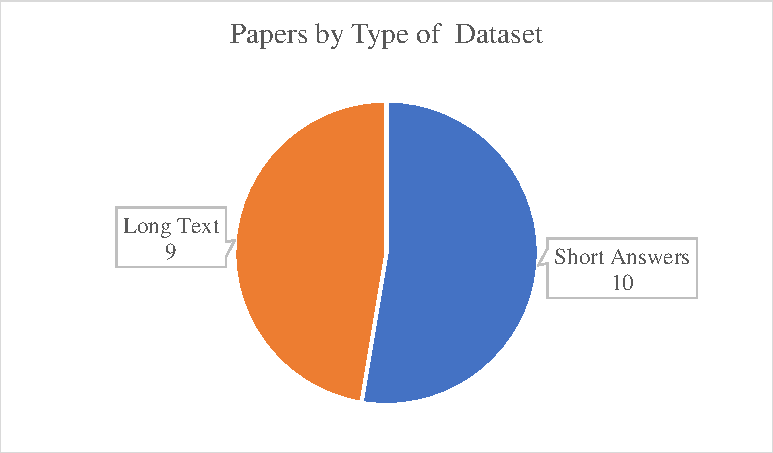
\includegraphics[width=0.5\linewidth]{img/papersbytype.pdf}
		\caption{Number of short Answer and number of long answer models}
		\label{shortlongcomparison}
	\end{figure}
	
	\subsubsection*{Text-to-Text Similarity Algorithms}
	Text similarity algorithms can be used to compare the student's answer with a model answer or answers from training dataset. This includes knowledge based similarity, string based, corpus based, and hybrid text similarity measures. They try to identify the degree of similarity between words based on the information extracted from the text. Hybrid uses different combines these measures to generate a similarity measure. Common measures used in papers dealt with either lexical similarity (similarity of characters) or semantic similarity (similarity of meaning).
	\begin{enumerate}
		\item Knowledge Based Similarity \\ Knowledge based uses semantic networks to assess the similarity of ideas between the text. Semantic networks are used for this approach. One database used for this is the WordNet. WordNet has its versions available in various languages, including Arabic, Hindi, Bengali and Persian. 
		\item Corpus Based \\ It uses information from large corpora to measure semantic similarity between words. A common corpus based technique is latent semantic analysis (LSA). This technique assumes that words with similar meaning will occur in similar portions of text. Term document matrix, a matrix of word counts per document, is made. Raw frequencies are often transformed using weighting schemes such as TF-IDF. It includes Term Frequency (TF): the number of occurrences of the term in the document, and Inverse Document Frequency (IDF).
		$$\text{TF}(t, d) = \frac{\text{Number of occurrences of term }t}{\text{Total number of occurrences in document }d} $$
		$$\text{IDF}(t, D) = \log \left( \frac{\text{Total number of Documents in the Corpus }D}{\text{Total occurrences of the term }t} \right) $$
		The weight $w$ is then determined by multiplying TF and IDF.
		It is followed by mathematical technique called Singular Value Decomposition (SVD), which lowers the rank of the term-document matrix. Matrices for both documents are then compared by cosine similarity. \\ One drawback of LSA is that it can be limited when dealing with contextual ambiguity. For example, ``bank" (as in a financial institution) and ``bank" (as in the side of a river) have different meanings but will be placed semantically close together in latent space. LSA also treats text as ``bag of words", meaning that it ignores the order of words in a sentence. For example, ``The dog chased the cat" and ``The cat chased the dog" would be treated similarly by LSA even though they have quite opposite meanings. Furthermore, the reliance on SVD makes it sensitive to quality and quantity of the input data. Therefore, it requires large, high quality training data. \\ Latent Semantic Indexing (LSI) is essentially an application of LSA and is primarily used for information retrieval purposes. \\ 
		\textbf{DISCO} (Extracting Distributionally similar words
		using CO-occurrences) is a tool developed by \href{https://www.linguatools.de/disco/disco_en.html}{Linguatools}. It extracts distributionally similar words by analyzing a large text corpus to gather co-occurrence data, where words are examined based on how frequently they appear together within a defined context window. It constructs co-occurrence matrices and uses similarity measures such as cosine similarity or Jacquard similarity to quantify the relationship between words. Finally, DISCO generates lists of similar words by ranking them based on their co-occurrence patterns and similarity scores. It currently supports Arabic, Czech, Dutch, English, French, German, Italian, Russian and Spanish.
		
		\item String-based Similarity \\ Judges similarity of two strings based on the character composition and string sequences. Some string based similarity measures used in our paper included:
		\begin{enumerate}[]
			\item Damerau-Levenshtein (DL) distance \\ It is the minimum number of operations required to turn string $S_1$ into string $S_2$, where the operations can be insertion, deletion, transposition of characters, or substitution of single character. Normalization \cite{1_gomaa2014arabic} is done to compute the similarity.
			\item Longest Common Substring (LCS) \\ It identifies the longest sequence of characters (substring) shared between two texts. Such scoring can be useful for determining whether key ideas and references are present.
			\item N-gram Similarity \\ An n-gram is a contiguous sequence of n items from a given text, where the items can be characters, words, or even phonemes. It is a sliding window approach that can be used on a character level or word level. First splits text into smaller units (n-grams) of different sizes. Then, the number of matching n-grams can be counted or jacquard similarity can be calculated.
			\begin{itemize}
				\item Jacquard Similarity \\ $$J(A,B) = \frac{|A \cap B|}{|A \cup B|}$$ Where $A \cap B$ is the number of n-grams common to both texts, and $A \cup B$ is the total number of unique n-grams in both texts.
			\end{itemize}
		\end{enumerate}
	\end{enumerate}
	\textbf{Text similarity and dissimilarity measures} \\
	These are statistical methods used to identify the degree of how two texts are alike. Higher the similarity, the more the texts are alike. The lower the dissimilarity, the more the texts are alike.
	\begin{itemize}
		\item Cosine Similarity \\ Given two vectors, it provides a cosine of the angle between those two vectors.
		$$S_c (t_1, t_2) = \frac{t_1 \cdot t_2}{|t_1||t_2|}$$ Where cosine similarity of text 1 and text 2 is the dot product of these vectors divided by product of magnitudes of those vectors. Value ranges from 0 (least resemblance) to 1 (most resemblance).
	\end{itemize}
	
	\subsection{Model Evaluation Metrics} 
	\subsubsection*{Kappa Score}
	Also known as the Cohen Kappa Statistic, can be used to measure the agreement of classification models. It is considered more reliable than a simple agreement measure because it can take into account the possibility of agreement by chance. \\ Observed agreement $P_o$ is the proportion of similar scores by human rater and the AES system. $P_e$ is the hypothetical chance of agreement, based purely on the probability of both raters randomly assigning the same score. 
	
	$$k = \frac{P_o - P_e}{1 - P_e}$$
	
	\subsubsection*{Quadratic Weighted Kappa}
	Weighted Kappa, not only takes the presence of agreement like Kappa does, but also takes into the seriousness of disagreement between raters as well. While Kappa is used for nominal variables, Weighted Kappa is used for ordinal variables (variables where the variables have ordered categories). \\
	After calculating $P_o$ and $P_e$ these values are multiplied by a weights matrix. The weight determines the seriousness of disagreement between human and AES rating. Weights can be measured linearly as well as in a quadratic form. A matrix of $n \times n$ for the expected frequency of pair ${i, j}$ and a matrix for observed frequency of pair $i, j$ are made. Here, $i, j$ are the scores by both raters. \\
	In order to determine the weight, the follow formula is used:
	$$W_{i, j} = 1 - \frac{|i - j|}{n - 1}$$
	$$W_{i, j} = 1 - \left( \frac{i - j}{n - 1} \right) ^2$$
	
	Here, n is the possible categories or number of possible ratings. Calculation of the weight will be dependent on $i - j$, where $i, j \in \{ 1, 2, 3, \dots n$ \}. The greater the difference in score, the smaller the weight will be. Majority of evaluations use Quadratic Weighted Kappa (QWK). \\
	Using the Weight $W$ matrix, Observed frequency matrix $O$, and Expected frequency matrix $E$, the score is measured:
	$$k_W = \frac{\sum_{i, j} W_{i, j} \cdot O_{i, j} - \sum_{i, j} W_{i, j} \cdot E_{i, j}}{1 - \sum_{i, j} W_{i, j} \cdot E_{i,j}}$$
	\subsubsection*{Precision}
	It is the proportion of correctly identified positive results out of all results that were predicted to be positive. In AES, precision measures how often the system's decision to assign a particular score (e.g., a high grade or a pass) was correct.
	$$\text{Precision} = \frac{\text{True Positives (TP)}}{\text{False Positives (FP) + True Positives (TP)}}$$
	\subsubsection*{Recall}
	It is the proportion of actual positive results that were correctly identified by the system. Recall measures how well the system captures all the relevant essays that should have been assigned a particular score (e.g., all essays deserving a high grade).
	$$\text{Recall} = \frac{\text{True Positives (TP)}}{\text{True Positives (TP) + False Negatives (FN)}}$$
	\subsubsection*{F-Score}
	It represents a weighted harmonic mean of precision and recall, where different weights can be assigned to precision and recall.
	$$F_\beta = (1 + \beta^2) \times \frac{\text{Precision}}{\beta^2 \times \text{Precision} + \text{Recall}}$$. Majority of papers used the $F_1$ score, where $\beta = 1$ (precision and recall are considered to be of equal importance).
	
	\subsection{Short Answer Scoring}
	
	%\subsubsection*{Hybrid Approaches}
	\textbf{\textcite{1_gomaa2014arabic}} (Arabic) combines string based, corpus based, and knowledge based similarity measures. String similarity is calculated using LCS (Longest Common Subsequence). They performed normalization tasks as well. They also calculated DL distance. They used character-based and word-based N-gram similarity was calculated and determined that character-based N-gram performed better in their model overall. 
	For corpus based measure, the paper utilizes DISCO. For measuring knowledge based similarity, the paper translated the dataset into English and the semantic similarity was measured through the English WordNet instead of the Arabic version, because of weak word coverage in the Arabic WordNet. They claimed translation helped improve the results of the model. An improved version of the Arabic WordNet, however, has been released since then. \\ They also introduced a sentence level semantic similarity measure. The system computed sentence-level semantic similarity using the Bag of Words model and they created a similarity matrix of word pairs between student and model answers. A matrix captured individual word similarities to calculate an overall score. \\ The paper showed a correlation between examiners of 0.86 and correlation between the model and examiner was 0.83. They also compared different translators and results showed human translation to be better than Bing or Google when applying string based similarity measures on translated text. Performance of Google and Bing translation was close to each other. They proposed a CombineBest method to determine the features that provided the best correlation and then used SMOReg (A variant of Support Vector Machine algorithm similar to \textcite{4_abdeljaber2021wordnet}) and Linear regression to obtain best Pearson correlation of 0.83. Best RMSE value of 0.75 was obtained by applying SMOReg on CombineBest method. In comparison, the Pearson correlation and RMSE between two annotators was 0.86 and 0.69 respectively. \\
	
	\textbf{\textcite{2_shalabi2016levenshtein}} (Arabic) uses a similar approach by first carrying out heavy stemming and then determining the weight of each word by calculating the Levenshtein (DL) distance. After determining the weights of the words in student answer, the model looks for presence of that word in the final answer. If there is some level of similarity, the weight of that word is added to the final score. The paper only dealt with string-based similarity measure. \\
	
	\textbf{\textcite{3_shehab2018arabicsimiliarity}} (Arabic) proposed a Bag of Words Model to determine the final score. The paper experiments with using Levenshtein (DL) distance and N-gram for  string similarity and LSA and DISCO for corpus based similarity measure. Their experimental results showed that N-gram based measures gave the highest correlation (0.820) out of the 4 similarity measures. DL was 2nd (0.800), and the corpus based measures DISCO and LSA were third (0.796) and fourth (0.796) respectively. \\
	
	\textbf{\textcite{8_abdel2021lcs}} (Arabic) uses LCS (longest common subsequence) 
	Arabic WordNet provides synonyms, which improves the accuracy of the model. The paper uses a modified approach of LCS using a weight based measurement technique.
	It also discusses the limits of Arabic WordNet due to limited coverage, so certain plural forms don't work in AWN. To deal with this issue, stem of model answer and stem of synonyms used to determine whether they lie in the common ``synset"
	
	The problem of standard LCS is that certain student answers can give a similar score with some model answers that are much closer to model answers syntactically. For this, the model not only uses contiguity of LCS for certain substrings in model answer and student answer, but also considers contiguity of all common subsequence of these texts. This turns the LCS to LCCS (longest common contiguous sequence) - The value for LCCS is also normalized. The final results obtained were $r$ of 0.94 and RMSE of 0.81. According to them, they were able to outperform other LCS models by utilizing Arabic WordNet as well as using LCCS instead of LCS. \\
	
	\textbf{\textcite{16_rababah2017short}} (Arabic) also applies LSA against a model answer. During their preprocessing, they aimed to improve the accuracy by presenting a hybrid method to verify the correctness of extracted stems by using multiple stemmers and WordNet. Their model consisted of making a term document matrix, applying TF-IDF to determine word weights, and measurement of score using cosine similarity. They achieved a 95.4\% percent correlation. They used a recall based approach (precision, accuracy, f-score) and found 62\% correlation when using R-call based scoring. \\
	
	\textbf{\textcite{27_gaheen2021jaya}} (Arabic) proposed a neural based approach. After preprocessing, a word by context (WCM) matrix is built to perform LSA. Then, they created a multi-layer perceptron network (MLP). Elitist-Jaya optimization algorithm was used to optimize the network. This process involved generating random vectors that are evaluated to optimize the neural network. They also experimented with various other optimization algorithms. The model achieved an average 0.987 correlation using eJaya, followed by DE (Differential evolution), MVO (Mean-Variance Optimization), and PSO (Particle Swarm Optimization). eJaya outperformed a conventional neural network by 7\% . 
	\subsubsection*{Feature Extraction using Support Vector Machine}
	Support Vector Machines (SVM) work by mapping data into a high-dimensional space, where each feature corresponds to an axis. A linear classifier is then trained by finding a hyperplane that separates positive and negative instances. The direction of this hyperplane is determined by the support vectors—key data points that define the decision boundary.
	
	Feature selection in SVM aims to retain only the most important features that contribute to accurate classification. One common method is the F-score, which evaluates how well each feature differentiates between two classes (positive and negative). Features with higher F-scores are considered more significant. Other methods, like Recursive Feature Elimination (RFE) or mutual information, can also be used to rank and select features based on their contribution to the model's performance. \\ 
	
	\textbf{\textcite{4_abdeljaber2021wordnet}} used SVM with F-score measure to select the important features to score short answers. In addition, it used the Arabic WordNet to determine synonyms. Finally, the score is generated using cosine similarity of model answer and student answer matrices. They achieved $r$ of 0.99 with Arabic WordNet and 0.98 without the WordNet.
	
	\subsubsection*{Transformer Approach in Short Answer Scoring}
	\textbf{\textcite{22_meccawy2023mining}} also experimented with different approaches. They used ARASAG and \textcite{16_rababah2017short}'s dataset. FARASA was used for light stemmming and ISRI stemmer was used for base stemming. One approach was to use the Arabic WordNet to consider synonyms and then semantic similarity by cosine similarity. The second approach was to utilize Word2Vec. It is a word embedding technique that presents words as vectors in a vector space and the closer the words are, the greater the similarity of their meanings. AraVec was used as the Word2Vec model. The third approach as to use BERT based approach, utilizing AraBERT. Cosine similarity was used for the similarity measure. Their methods performed better overall when using light stemming. The best RMSE achieved was through BERT (1.04), which was significantly better than any other method. Best $r$ was obtained by using Word2Vec (0.78) in ARASAG dataset. The same model, when trained and applied on the Rababah's dataset, achieved greater $r$ (0.84) and performed slightly better with base stemming approach. \\
	
	
	\textbf{\textcite{23_ghazawi2024bert}} has introduced AR-RES, one of the largest publicly available datasets for Arabic AES. The dataset consists of questions and answers from different topics, divided by genders as well. They utilized ISRI stemmer for their preprocessing and the AraBERT tokenizer for tokens. After training the model on AraBERT their model achieved a QWK score of 0.884 and an F1 score of 0.78. The performance of their model exceeded in some topics than others. They explained this to be because of the complexity of certain topics: the model showed lower performance in topics like Management Information Systems, where the course had more open-ended answers while answers in courses like Chemistry were source dependent and controller and therefore the model performed better. 
	
	\subsection{Long Text Essay Scoring}
	\subsubsection*{Measure of Coherence with Discourse Analysis}
	Two common methods to determine coherency of an essay are Rhetorical Structure Theory (RST) and Segmented Discourse Representation Theory (SDRT). \\ In RST, texts are divided into segments called "nuclei" (central ideas) and "satellites" (supporting ideas), which are connected through rhetorical relations, such as cause-effect, contrast, or elaboration. These relations describe how different sections of a text interact to form a cohesive argument or narrative. 
	
	\textbf{\textcite{6_ghamdi2014hybridarabic}} (Arabic) presented Abbir, a hybrid AEE for essays in Arabic language. They built an LSA concept space and also measured surface level features by measuring spelling mistakes and number of words. In the training phase, the LSA concept space was built using a training dataset and the LSA distance. Best result achieved by including LSA with stemming, word distance, and spelling mistake distance was $r$ of 0.78 and RMSE of 0.89. Their threshold value $t$ was set to be 17\% of the overall score. 
	
	\subsubsection*{Rule based approaches}
	\textbf{\textcite{7_qahtani2019rulebased}} used MADAMIRA \cite{pasha2014madamira} for morphological analysis during preprocessing for part-of-speech tagging and stemming words. Spelling errors were identified using FARASA spell checker. The paper also considers structure of essay by considering the essay to be divided into introduction, main body, and conclusion. Coherence of the answers was measured by counting discourse connectives. They also measured checked for punctuation marks and style level by counting frequency of repeated words. Threshold was set for 16\% of the overall score. 73\% of the scores were considered to be within acceptable range.
	
	
	\subsubsection*{Transformer Model and Deep Learning approaches}
	Text classification is difficult in many such languages because of the lack of available scored datasets. This is where, the deep learning method can help address such problems. One of the significant advantages of using transformer architecture over deep learning models is that they are less susceptible to vanishing gradient problem. They rely on attention mechanism rather than sequential processing used in RNNs or LSTMs. They are able to capture relations of text input in context to other text inputs. \\
	
	
	\textit{BERT} \\
	Bidirectional Encoder Representations from Transformers is an open-source machine learning framework utilized in many NLP applications. It uses a transformer based neural network to generate human-like language. A conventional transformer model consists of encode and decoder modules but BERT has an encoder-only architecture, meaning it works mainly in understanding the input sequences rather than generating the output. \\ BERT is pretrained on large amount of unlabelled data, where it learns contextual embeddings. It can be fine by training on labelled data. \\ While traditional models work by processing text in one direction, BERT works by using a bidirectional approach: The model analyzes the text from both directions. This way, it is able to generate embeddings that are deeply contextualized. Improved model understanding allows for better assessment of coherence, relevance and precision of arguments in an essay. Since such architecture can capture more comprehensive context, it can be better at generalizing different writing styles and improve reliability of the scoring in comparison to unidirectional encoder. It uses MLM (masked language model) and next sentence prediction when training in order to easily define a prediction goal. RoBERTa also uses self-attention to evaluate input sequences and construct phrase-level contextual representations. It is arguably more effective because it is primarily trained on a larger dataset (160gb) in comparison to BERT (16GB) \\
	
	\textbf{\textcite{9_firoozi2024bert}} (Persian) uses multilingual BERT (mBERT) to score long essays. First they built a model using a Word Embedding Model using Word2Vec. In Word2Vec, words are represented as vectors of real numbers, where semantically similar words have similar vector representations. This model was used for comparison against mBERT model. After fine tuning the mBERT, they were able to achieve kappa score, QWK and accuracy of 0.93, 0.84, and 73\% respectively. This was significantly better than the word embedding model where they achieved Kappa score, QWK and accuracy of 0.82, 0.75 and 71\% respectively. Their model performed well with various levels of text difficulty but the performance dropped in grading advanced level essays. \\
	
	
	\textit{Deep learning and LSTM} \\
	Long short term memory, usually employed in preprocessing stage, used for semantic analysis. This architecture helps model to recognize the temporal dependencies and patterns within the text data. LSTM can provide unique strengths when dealing with long texts consisting of sequential data. It is a type of recurrent neural network (RNN) that aims to solve the vanishing gradient problem in neural networks. Hence it plays a key role in capturing long-range dependencies in the data. LSTMs have a memory cell that can store and retrieve information over long periods of time. Hence not only storing relationships between words and certain phrases but also flow of ideas in a response. \\
	
	\textbf{\textcite{10_singh2023hindi}} (Hindi) thoroughly documented the various approaches for their model. They experimented with Linear Regression, Support Vector Regression (SVR), RandomForest and XGBoost for classification and regression approach. They extracted features like essay length, average word length, readability, vocabulary, and semantic overlap and coherence. They calculated readability scores using \cite{sinha2012new} and vocabulary score by counting out-of-vocabulary words. mBERT is used to measure semantic similarity of two sentences at a distance of four sentences. \\ For building a neural-network based architecture,  they experimented with a total of 4 neural-based approaches. \\ The BiLSTM method consists of two LSTMs processing the sequence in both forward and backwards direction. CNN (Convolutional Neural Network) was used to capture short dependencies over a fixed window size. The also combined CNN to extract features from the text and then used LSTM for to process sequences. They attached an attention layer to it. Their fourth neural approach was to implement SKIPFLOW Model \cite{tay2018skipflow}. This novel approach calculates coherence by reading LSTM networks. \\ They also fine tuned a number of transformer models: Multilingual BERT (mBERT), DistilmBERT, XLM-Roberta, MuRIL, and IndicBERT. Their dataset consisted of both an organic corpus and a translated corpus from the ASAP dataset. Overall, their methods were able to show more consistent results with translated texts. From regression appraoches, XGBoost provided the best results with QWK score of 0.827 in organic corpus. Different regression approaches had a large variation in their QWK scores (0.579 - 0.827) when working in organic corpus. Neural based approaches, however, had a higher average with BiLSTM providing the best results (0.842) followed by CNN + LSTM + Transformer (0.827) and SKIPFLOW (0.812). Transformer based models were able to provide the best results with mBERT scoring 0.852: highest for evaluating organic corpus. \\
	
	\textbf{\textcite{11_walia2024hybrid}} (Hindi) used a similar approach to \textcite{10_singh2023hindi}, utilizing LSTM and a transformer model. They implemented a Hybrid PSO (Particle Swarm Optimization) based approach for LSTM and RoBERTa. The model achieved an overall accuracy of 95\%. Details of the datasets, however, were not shared.
	
	\subsubsection*{Information Retrieval Approaches}
	\textbf{\textcite{17_abbas2015svm}} focuses on VSM and Latent Semantic Indexing in web-based learning. Information retrieval (IR) is applied to extract information from the text. Each query for IR  The idea behind VSM is to represent each essay as a vector as a point in space. \\ Similarity between the vector and the query is done through matching functions. The model generates an vector for each essay and for each query from sets of terms with their weights. The weight of each term is identified through TF-IDF. Then, the cosine similarity between the vector for the query and the vector of the essay is measured. \\ In the second stage of the model, they implemented LSI, where they built the term document matrix. Instead of performing SVD, they performed truncated SVD, which they claimed, could help reduce noise and remove unnecessary information for their application. The result for the LSI score is found by cosine similarity between the LSI vector (after truncated SVD) and a query (vector consisted of terms for the query). As new documents get added to the LSI space, the term document matrix needs to be recalculated. Instead of rebuilding the matrix from scratch, they suggested folding in to reconstruct the matrix. The final score generated was the average of the VSM score and the LSI score. The dataset used in the study was not large, consisting of 30 essays. Their model correctly scored 23/30 essays. They achieved a correlation of 0.978. \\
	
	
	\textbf{\textcite{24_islam2013abess}} (Bengali) also built a model utilizing information retrieval and GLSA (generalized latent semantic analysis). They created an n-gram document matrix by first determining the index terms. The n-grams are weighted by multiplication of frequency of n-grams by n. Then, SVD is carried out on the n-gram document matrix. A query matrix is created from a submitted essay and cosine similarity of the query vector with with term-document matrix determines the grade. They achieved precision and recall of 98\%. 
	
	\subsubsection*{Hybrid Approaches in long essay systems}
	\textbf{\textcite{5_aljouie2017schoolchildren}} uses LSA of the student answer against the training dataset. It uses RST to determine 40\% of the score, LSA for 50\% of the score, and 10\% of the score is measured by spelling mistakes. \\ They set the threshold to be 1.5 marks and achieved an accuracy of 78.33\% \\
	
	
	\textbf{\textcite{18_alqahtani2020svr}} categorized the features extracted from the text into surface level (quantitative measures for counting words), syntactic (presence of POS and mistakes), lexical (presence of certain keywords, punctuation features etc.), semantic (using Arabic WordNet and word embedding) and discourse (identifying discourse connectives). In the first part of the paper they presented a thorough list of features that they were able to extract from the text. In the second part of their paper, they proposed 4 models.
	\begin{enumerate}
		\item Spelling model. Necessary features were identified and the FARASA spell checker was used. They also assessed the performance of FARASA on their dataset where there was cases where it failed to correct the mistake (3.4\%) or corrected a word that was already correct (10.1\%). At $t = 17\%$ and $t = 25\%$, it achieved $r$ of 0.65, 0.72 respectively.
		\item Structure model identified structure of the text using surface level and some lexical features like presence of keywords. At $t = 17\%$ and $t = 25\%$, it achieved $r$ of 0.74, 0.86 respectively.
		\item Coherence model used discourse features and surface level features to identify how well the sentences are linked together. At $t = 17\%$ and $t = 25\%$, it achieved $r$ of 0.65, 0.69 respectively.
		\item Style model uses morphological and surface level features to find word repetition, number of synonyms, number of discourse connectives. At $t = 17\%$ and $t = 25\%$, it achieved $r$ of 0.57, 0.65 respectively.
		\item Punctuation marks model used punctuation and discourse features to determine correct usage of marks. At $t = 17\%$ and $t = 25\%$, it achieved accuracy of 90\% and 96\% respectively. 
	\end{enumerate}
	Overall, the model achieved 96\% accuracy and 0.87 correlation. \\
	\textbf{\textcite{26_alsanie2022threelevels}} worked by improving the existing model by \textcite{6_ghamdi2014hybridarabic}. The model evaluated the essay’s style in terms of syntactic structure and spelling, while analyzing its content through lexical semantics. A context-free grammar model was employed; however, due to the need for language contextualization and the difficulty in distinguishing between salient and anomalous language constructs, the model was lexicalized and enhanced with probabilistic rule choices, converting it into a stochastic lexicalized context-free grammar. Sub-tree kernels and Support Vector Machines (SVMs) were used for syntactic measurements, with flexibility in the SVM to account for dataset uncertainty. Latent Semantic Analysis (LSA) was also applied, and logistic regression was used to determine the final score. The model outperformed \textcite{6_ghamdi2014hybridarabic} and achieved best QWK of 0.68 and accuracy of 51\% while \textcite{6_ghamdi2014hybridarabic}'s model achieved best QWK and accuracy of 0.34 and 44\%, respectively.
	
	
	\section{Discussion}
	
	\begin{center}
		\begin{tikzpicture}[
			level 1/.style={sibling distance=28em, level distance=5em},
			edge from parent/.style={draw, -latex, edge from parent path={
					(\tikzparentnode.south) -- ++(0,-1.2em) -| (\tikzchildnode.north)}},
			every node/.style = {shape=rectangle, rounded corners,
				draw, align=center, fill=white, inner sep=1em}
			]
			
			% Root node (top of the hierarchy)
			\node {AES Methods}
			child { node {Short Answer (10)} }  % First child
			child { node {Long Text (9)} };     % Second child
			
		\end{tikzpicture}
	\end{center}
	
	\begin{table}[H]
		\begin{tabularx}{7in}{|X|m{0.8in}|m{0.8in}|}
			\hline
			\multirow{2}{*}{Common Approaches} & \multicolumn{2}{c|}{Number of papers} \\ \cline{2-3}
			& Short Answer & Long Text \\ \hline
			String Based Similarity (Including N-gram, LCS, DL Distance) & 8 & 1 \\
			Corpus Based Similarity (Including LSA, LSI, DISCO) & 6 & 3 \\
			Knowledge Based Similarity (Utilizing WordNet for Synonyms) & 4 & 1 \\
			Support Vector Machines (Including classification and regression) & 2 & 3 \\
			Transformer Models & 2 & 3 \\
			Neural Based Approaches & 1 & 2 \\ 
			\hline
		\end{tabularx}
		\caption{Number of Papers Utilizing Each Method}
		\label{tab::papertypes}
	\end{table}
	Table \ref{tab::papertypes} the number of papers that assessed and used a certain technique in their paper. The table also considers papers that used multiple approaches. While string based methods were computationally efficient they did not capture semantic meaning. Therefore, majority of papers utilized this approach alongside a semantic measure. \\ Many papers used Latent Semantic Analysis (LSA) as a key method to measure corpus based similarity. Since LSA is built using a term-document matrix, where the matrix represents the frequency of terms across a set of documents, LSA and its extension Latent Semantic Indexing (LSI) typically require reprocessing the entire matrix and recalculating the singular value decomposition (SVD) matrix. If the matrix is large, this operation can be computationally expensive, posing a significant challenge when dealing with large-scale datasets. In comparison, scalable approaches using deep learning and transformer models, such as BERT and GPT, may help resolve this problem by handling semantic relationships more effectively without relying on explicit matrix factorization.
	
	\textcite{17_abbas2015svm} proposed a workaround to LSA’s computational limitations by employing a "folding-in" method. Instead of recalculating the entire SVD from scratch whenever a new essay is added, the new essay was mapped into the existing LSA space by projecting it onto the original SVD components. This significantly reduced the computational overhead.
	
	LSA’s bag-of-words nature leads to another limitation: it cannot capture word order or syntactic nuances. This inability to differentiate between sentences that contain the same words but in a different order can affect the accuracy of the model, particularly in cases where student answers might use similar words as the model answer but convey completely different meanings. For example, "The essay argues against X" versus "The essay argues for X" would be treated similarly by an LSA-based system, despite the opposite meanings conveyed.
	
	To mitigate some of these issues, \textcite{26_alsanie2022threelevels} utilized a parser algorithm in combination with LSA to analyze sentence structure and dependencies, allowing for a more refined assessment of the essay’s content.
	
	Recent advances in AES have moved towards the use of deep learning models, particularly those based on neural networks and transformers, which can better account for word order, context, and semantic relationships. 
	
	Support Vector Machines (SVM) have been utilized for both classification and regression tasks in AES, particularly in systems that involve scoring rubrics. SVMs are well-suited for tasks where the feature space is relatively well-defined, such as specific grading categories (e.g., grammar, coherence). However, the performance of SVMs can degrade when the feature space is large or noisy, which is often the case in long-text essays that contain diverse expressions and stylistic variations. To account for these challenges, some studies have proposed less rigid implementations of SVM \cite{17_abbas2015svm}, allowing for greater flexibility in the presence of dataset uncertainty.
	
	Transformer models, using BERT and its variants, pre-trained on large text corpora, have the advantage of being more scalable, as they can process text in a parallelized manner and fine-tune on essay-specific tasks. The multilingual models can be applied in various applications which can make the technique more transferable than others. However, training them is resource intensive and requires a large corpus. Currently, the performance of BERT was assessed by \textcite{9_firoozi2024bert} and showed a drop in performance when assessing advanced level essays. 
	
	\section{Conclusion}
	
	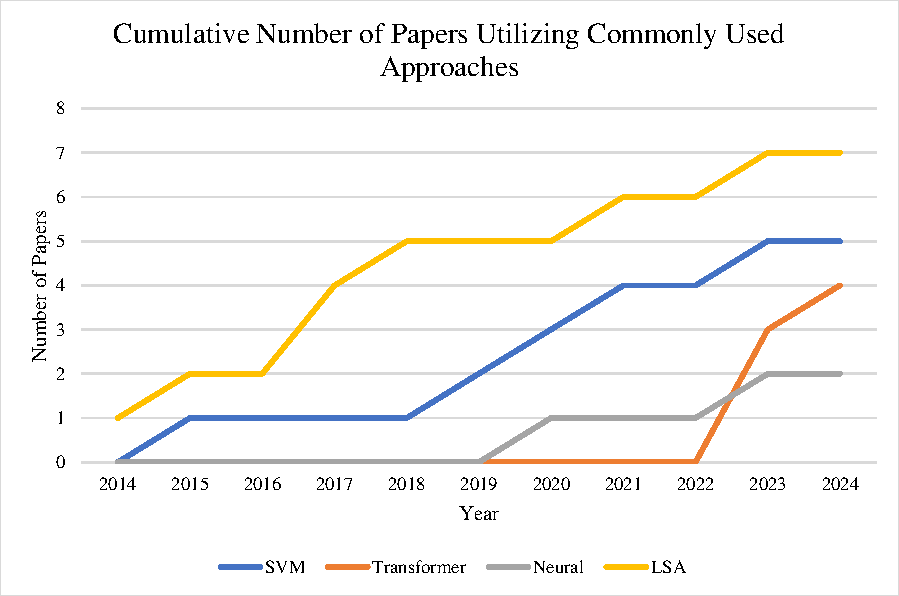
\includegraphics{img/paperstrend.pdf}
	
	To conclude, the future of AES for low-resource languages looks promising, though there are challenges to overcome. The primary challenge is the limited availability of training datasets. The graph shows that traditional techniques, such as corpus-based similarity methods like LSA, have been prevalent over time. However, with the introduction of transformer architectures, there has been a noticeable rise in deep learning and transformer-based approaches due to their superior ability to measure semantics. We hope that ongoing advancements will make these powerful models more accessible and effective for low-resource languages, ultimately improving the accuracy and fairness of AES systems across diverse linguistic contexts.
	
	Certainly, coupling scores with feedback is crucial for learners. It is necessary to provide more detailed explanations for the scores attributed, as this can greatly enhance the learning experience. A significant drawback observed in the literature is the lack of feedback and explanations accompanying the grades. Many studies had to rely on translating datasets instead of using organic corpora, which could affect the quality of the results. The general scarcity of datasets further exacerbates these issues. Addressing these concerns by integrating detailed feedback and improving dataset availability will be essential for developing more effective and equitable AES systems.
	
	% \bibliographystyle{IEEEtran}
	\printbibliography
	% \bibliography{ref.bib}
\end{document}
